\begin{questions}
\question{
No 5-fold symmetry
}
\begin{solution} The short answer to why there is no 5-fold symmetries in crystals is, because we can not cover a plane (space) entirely using only regular pentagons.

We can also show an interesting proof using a shrinking argument. We know that a rotation symmetry must move a lattice point to a succession of other lattice points. In other words, a rotation must move lattice points to other lattice points. Now let's set up our rotations

\begin{center}
  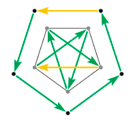
\includegraphics[width=45mm]{shrink}
\end{center}

\captionof{figure}{Translation vectors for a $2\pi/5$ rotation in a ``pentagonal lattice''. Taken from \textit{http://enacademic.com/dic.nsf/enwiki/1056789}.}\label{shrink} \vspace{0.5cm}

If a displacement exists between any two lattice points, then that displacement must repeat in every point of the lattice. Now let's take a point and construct a 5-point star joining the displacement vectors head to tail. As we know, all this points must be lattice points, but now the pentagon is smaller, and this cannot be possible, because this implies that the new ``shrinked'' points were also lattice points. We can repeat this process again and again until we can make the lattice points as close as we want, therefore modifying the lattice. If we had a rotation symmetry this wouldn't be possible, since the lattice under such rotations should be exactly the same. Therefore proving that a 5-fold symmetry is indeed impossible. $_\blacksquare$


\end{solution}

\question{Quasicrystalls}
\begin{solution}
  Quasicrystals are physical lattices with translational disorder that retain local, rotational symmetry. This means that crystalls have rotational and translational symmetries, while quasycristalls only have rotational symmetry, so if we move the lattice, the translated lattice will not match the original one.
\end{solution}
\end{questions}

%
% \begin{center}
%   \includegraphics[width=55mm]{}
% \end{center}
%
% \captionof{figure}{}\label{new}\vspace{0.5cm}
